% begin module limits-ex9
\begin{frame}
\begin{example} %[Example 1, p. 126]
Find $\lim_{x\rightarrow 3^+} \frac{2x}{x-3}$ and $\lim_{x\rightarrow 3^-}\frac{2x}{x-3}$.
\begin{columns}[c]
\column{.42\textwidth}
\ \ \uncover<4->{
$\lim_{x\rightarrow 3^+}2x/(x-3) = \infty$.
}

\ \ \uncover<7->{
$\lim_{x\rightarrow 3^-}2x/(x-3) =-\infty$.
}

\uncover<8->{%
\psset{xunit=0.14cm, yunit=0.14cm}
\begin{pspicture}(-3.1,-12)(18.5,33.3) \psframe*[linecolor=white](-3.1,-12)(30.5,33.3) 
\psaxes[ticks=none, labels=none]{<->}(0,0)(-3.1,-4.5)(30,30)
\psplot[linecolor=red, plotpoints=1000]{3.2}{30}{x 2 mul x -3 add div }
\psplot[linecolor=red, plotpoints=1000]{-3}{2.6}{x 2 mul x -3 add div }
\psline(-0.3,5)(0.3,5)
\rput(-1, 5){$5$}
\psline[linestyle=dotted](3, -12)(3,33)
\rput(10, 10){$y=\frac{2x}{x-3}$}
\rput[lt](3, -4){$x=3$}
\end{pspicture} 
%\uncover<8->{%
%\ \ 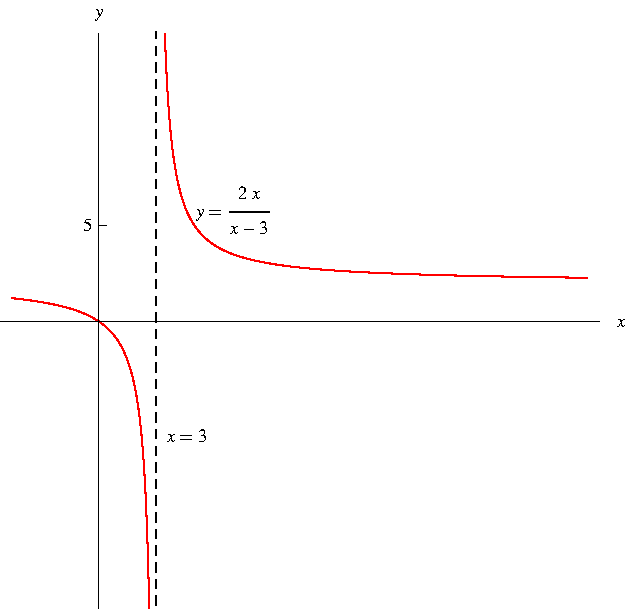
\includegraphics[height=5cm]{limits/pictures/02-02-ex9.pdf}%
%}%
}%
\column{.58\textwidth}
\begin{itemize}
\item<2->  If $x$ is near 3 but larger than 3, the denominator $x-3$ is a small positive number and $2x$ is close to 6.
\item<3->  So the quotient $2x/(x-3)$ is a large positive number.
\item<5->  If $x$ is near 3 but smaller than 3, the denominator $x-3$ is a negative number with small absolute value and $2x$ is close to 6.
\item<6->  So  $2x/(x-3)$ is a negative number with large absolute value.
\item<8->  $x = 3$ is a vertical asymptote for $f(x) = 2x/(x-3)$.
\end{itemize}
\end{columns}
\end{example}
\end{frame}
% end module limits-ex9
